\documentclass[12pt]{beamer}
\mode<presentation>
\definecolor{pjwgreen}{rgb}{0.196,0.349,0.157}
\usetheme{Frankfurt}
\setbeamercolor*{palette primary}{fg=white,bg=pjwgreen}
\setbeamercolor*{palette secondary}{fg=white,bg=pjwgreen}
\setbeamercolor*{palette tertiary}{fg=white,bg=pjwgreen}
\setbeamercolor*{palette quaternary}{fg=white,bg=pjwgreen}
\setbeamercolor{structure}{fg=pjwgreen}\setbeamercolor{local
structure}{parent=structure}

\usepackage[utf8]{inputenc}
\usepackage[polish]{babel}
\usepackage{polski}
\usepackage{amsmath}
\usepackage{amsfonts}
\usepackage{amssymb}
\usepackage{graphicx}
\usepackage{wrapfig}
\usefonttheme{professionalfonts}

\newcommand\Fontvi{\fontsize{14pt}{7.2}\selectfont}

\author{Paweł J. Wal\\Opiekun pracy: dr inż. Łukasz Rauch}
\title[Implementacja solwera frontalnego...]{Implementacja solwera frontalnego zrównoleglonego w wielowęzłowym heterogenicznym środowisku sprzętowym}
\institute[AGH]{
  Wydział Inżynierii Metali i Informatyki Przemysłowej\\
  Akademia Górniczo-Hutnicza im. Stanisława Staszica w Krakowie
}

\setbeamercovered{transparent} 
\setbeamertemplate{navigation symbols}{} 
\logo{} 
\date{7 maja 2015} 
%\subject{} 
\begin{document}

\begin{frame}
\titlepage
\hspace{80pt}

\includegraphics[scale=0.20]{logo_ms}
\end{frame}

\section{Motywacja pracy}
\subsection{Oryginalny pomysł - solwer multifrontalny na GPU}

\begin{frame}{Oryginalny pomysł - solwer multifrontalny na GPU}
\begin{itemize}
	\item Wykorzystany OpenCL
	\item Masowo równoległe przetwarzanie na GPU
\end{itemize}
\vspace{10pt}
\begin{itemize}
	\item Wydzielenie frontów rozwiązania
	\begin{itemize}
	    \item Podział macierzy na części (dekompozycja)
	    \item Wydzielenie z macierzy rzadkiej gęstych fragmentów
	\end{itemize}
	\item Przetworzenie frontów rozwiązania
	\begin{itemize}
    	\item Przetwarzanie części niezależnie od siebie
	    \item Rozwiązanie zależności - na koniec
	\end{itemize}
\end{itemize}
\end{frame}

\subsection{Oryginalny pomysł - dekompozycja}

\begin{frame}{Oryginalny pomysł - dekompozycja}
\begin{center}
	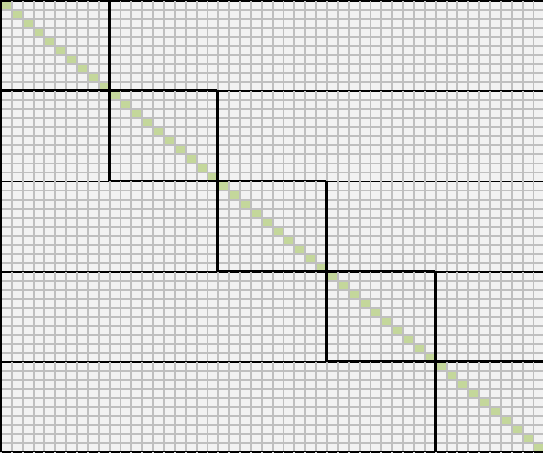
\includegraphics[scale=0.4]{dekompozycja}
\end{center}
\end{frame}

\subsection{Wady oryginalnego podejścia}
\begin{frame}{Wady oryginalnego podejścia}
\begin{itemize}
	\item Użycie tylko jednego z dostępnych urządzeń
	\item Uwarunkowania pamięciowe
	\begin{itemize}
	    \item Ładowanie stosunkowo dużych fragmentów macierzy do pamięci
	    \item Dodatkowa pamięć potrzebna na specyficzne struktury danych używane przez solwer (mapowanie wierszy)
	\end{itemize}
	\item Niewielka odporność na zdarzenia katastrofalne (np. awarię zasilania)
	
\end{itemize}
\end{frame}

\subsection{Nowy kierunek}
\begin{frame}{Nowy kierunek}
\begin{itemize}
	\item Użycie wszystkich dostępnych urządzeń
	\item Wykorzystanie możliwości maszyn z wieloma GPU?
	\begin{itemize}
	    \item Wiele GPU = specjalne płyty główne i obudowy = koszt
	    \item Wiele GPU = specjalne systemy operacyjne i konfiguracje = maszyna o wąskim zastosowaniu
	    \item Potęga GPU = moc urządzeń klasy konsumenckiej
	\end{itemize}
	\item Myśl przewodnia: realne zastosowanie w przemyśle i nauce	
\end{itemize}
\end{frame}

\section{Koncepcja}
\subsection{Założenia projektu}
\begin{frame}{Założenia projektu}
\begin{itemize}
	\item Możliwość wykorzystania dziesiątek, setek, ... urządzeń dowolnej klasy - przez OpenCL
	\item Dowolna lokalizacja urządzeń
	\item Dowolne dopuszczalne obciążenie urządzeń
	\item Brak nierealistycznych lub wygórowanych założeń (najlepiej: brak założeń w ogóle):
	\begin{itemize}
		\item Ilość urządzeń w maszynie
		\item Moc obliczeniowa urządzeń
		\item Rodzaj i jakość połączenia (filtrowane, komórkowe)
		\item Czas i wydajność pracy	
	\end{itemize}
\end{itemize}
\end{frame}

\subsection{Założenia projektu}
\begin{frame}{Założenia projektu}
\begin{itemize}
	\item Rozwiązywanie wielu problemów na raz
	\item Rozwiązywanie problemów uprzednio praktycznie nierozwiązalnych
	\item Odporność na błędy - od drobnych do katastrofalnych
\end{itemize}
\end{frame}

\subsection{Inspiracja}
\begin{frame}{Inspiracja}
\begin{center}

\includegraphics[scale=0.30]{sah_logo}\\ \vspace{25pt}

\includegraphics[scale=0.20]{boinc_logo} \\ \vspace{25pt}

\includegraphics[scale=0.40]{folding_logo}
\end{center}
\end{frame}

\subsection{Schemta rozwiązania}
\begin{frame}{Schemat rozwiązania}
\begin{center}
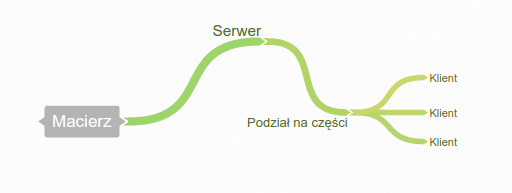
\includegraphics[scale=0.60]{schemta}\\ \vspace{25pt}
\end{center}
\end{frame}

\subsection{Przewaga rozwiązania}
\begin{frame}{Przewaga rozwiązania}
\begin{itemize}
\item Wykorzystanie ukrytego (marnowanego) potencjału urządzeń
\item Niewielkie wymagania własne 
\begin{itemize}
	\item Pracuje z dostępnymi technologiami i popularnymi urządzeniami
	\item Nie wymaga inwestycji
	\item Nie wymaga specjalistycznej wiedzy by być skutecznie użytkowanym
\end{itemize}
\item Pozwala na rozwiązywanie problemów niepraktycznych lub niemożliwych do rozwiązania
\end{itemize}
\end{frame}

\section{Realizacja}
\subsection{Architektura}
\begin{frame}{Architektura}
\begin{itemize}
	\item Klient-serwer
	\item Dlaczego nie MPI?
	\begin{itemize}
		\item Rozłączne LANy
		\item Pojedyncze maszyny w różnych lokalizacjach
		\item Gorsze połączenia
	\end{itemize}
	\item Ostateczna decyzja? Protokół HTTP!
	\begin{itemize}
		\item Popularność
		\item Typowość - raczej nie jest blokowany
	\end{itemize}
\end{itemize}
\end{frame}

\subsection{Serwer}
\begin{frame}{Serwer}
\begin{itemize}
	\item Ruby on Rails
	\begin{itemize}
		\item Jednolite, standardowe API (REST)
		\item Bezstanowość
		\begin{itemize}
		\item Rozwiązanie wielu problemów na raz
		\item Odporność na awarie nagle zatrzymujące serwer
		\end{itemize}
		\item Ta sama usługa dostarcza punkt wejścia dla klientów i dla użytkowników (interfejs graficzny)
	\end{itemize}
	\item Interfejs użytkownika
	\begin{itemize}
		\item Nowoczesne technologie webowe
		\item Łatwość obsługi - nawet dla laika
		\item W praktyce: kolejna redukcja kosztów (specjaliści, szkolenia, ...)
	\end{itemize}
\end{itemize}
\end{frame}

\subsection{Serwer - interfejs użytkownika}
\begin{frame}{Serwer - interfejs użytkownika}
\begin{center}
	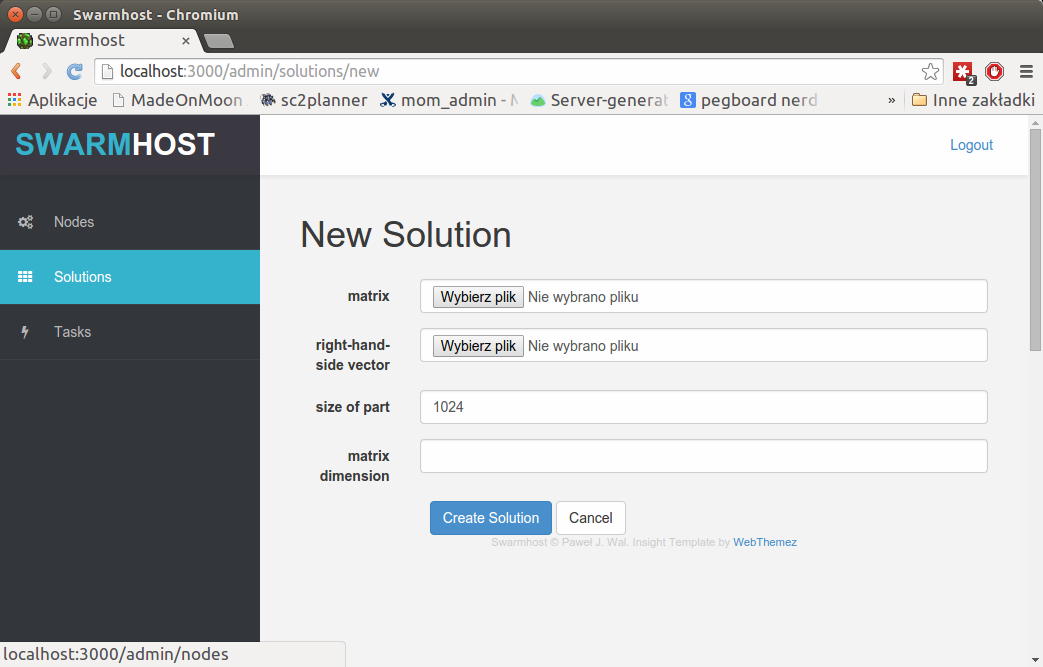
\includegraphics[scale=0.3]{swarmhost}
\end{center}
\end{frame}

\begin{frame}{Serwer - interfejs użytkownika}
\begin{center}
	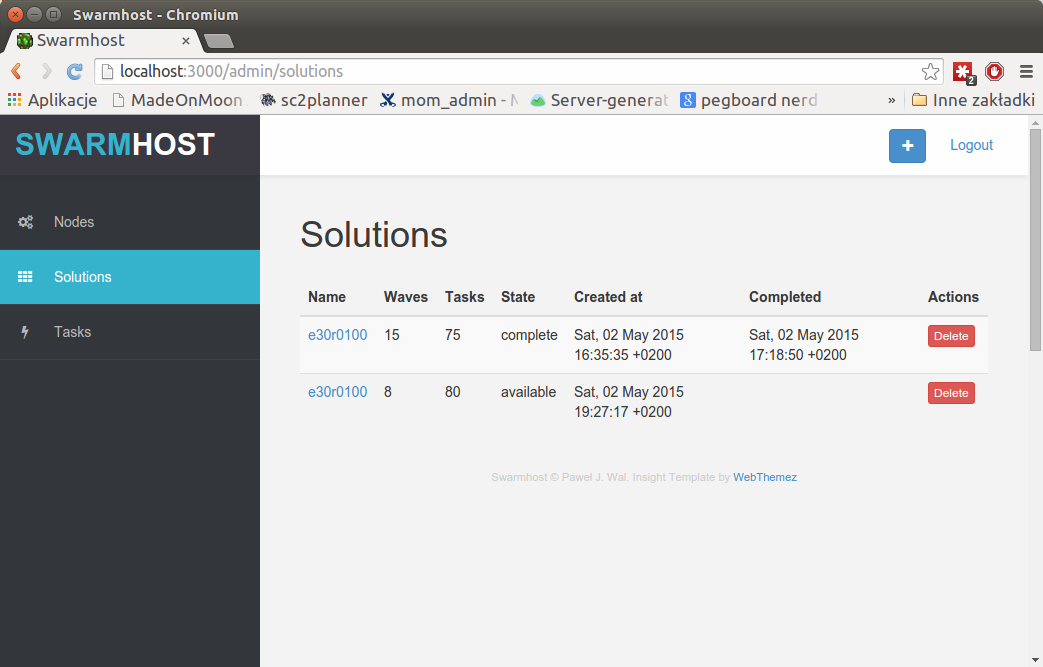
\includegraphics[scale=0.3]{swarmhost2}
\end{center}
\end{frame}

\subsection{Klient}
\begin{frame}{Klient}
\begin{itemize}
	\item Ruby
	\begin{itemize}
		\item Łatwość prototypowania
		\item Dynamiczny rozwój oprogramowania
	\end{itemize}
	\item Usługa rezydentna
	\begin{itemize}
		\item Pracuje tylko wtedy kiedy serwer podaje zadania
		\item Niewielki narzut ze strony samego klienta
	\end{itemize}
	\item Pełna asynchroniczność
\end{itemize}
\end{frame}

\subsection{Elementy obliczeniowe}
\begin{frame}{Elementy obliczeniowe}

\begin{columns}[T]
    \begin{column}{.7\textwidth}
\begin{itemize}
\item Trudno przebić C/C++
\begin{itemize}
	\item Szybkość
	\item Obsługa pamięci
	\item Dostępność bibliotek numerycznych (np. Boost C++ uBLAS)
\end{itemize}
\item Rozwiązanie: \\Ruby Native Extensions
\begin{itemize}
	\item Uruchomienie kodu natywnego w kontekście Ruby
	\item Rozwiązanie hybrydowe
\end{itemize}
\end{itemize}
    
 \end{column}
    \begin{column}{.3\textwidth}
    \begin{center}

\includegraphics[scale=0.3]{ruby_c}
\end{center}
 \end{column}
 \end{columns}
\end{frame}

\subsection{Zysk z użytych technologii}
\begin{frame}{Zysk z użytych technologii}
\begin{itemize}
	\item Łatwość rozszerzania serwera - prosty język,\\ jasna struktura danych
	\item Łatwość modyfikacji klienta
	\item Łatwość stworzenia zupełnie nowego klienta
	\item Cały dynamizm Ruby, cała szybkość C++, cała moc OpenCL i GPU
	\item Łatwość dostosowania do aktualnie postawionego celu przez specjalistę
	\item Łatwość użycia jako gotowego rozwiązania przez specjalistę w innej dziedzinie
\end{itemize}
\end{frame}

\section{Dalszy rozwój}
\subsection{Realizacja}
\begin{frame}{Dalszy rozwój}
\begin{itemize}
	\item Rozwiązanie jest nadal w rozwoju
	\item Aktualnie badane obszary:
	\begin{itemize}
		\item Usprawnienie komunikacji po HTTP
		\item Obniżenie obciążenia serwera
		\item Zwiększenie asynchroniczności kluczowych elementów
		\item Badanie wpływu parametrów podziału macierzy na prędkość uzyskiwania wyników
		\item Badanie wpływu parametrów uruchomieniowych OpenCL na szybkość uzyskiwania rozwiązań na kliencie
		\item I inne.
	\end{itemize}
\end{itemize}
\end{frame}


\end{document}